\subsection{Изолирующий лес. Расширение Deep IForest}

Изолирующий лес (Isolation Forest или IForest) --- это метод машинного обучения без учителя, основанный на принципе, что аномалии обычно редки и хорошо выделяются, что упрощает их идентификацию. IForest основан на идее разделения пространства признаков для обнаружения аномалий. Однако, в отличие от деревьев решений, где разделение основано на информации, в IForest процесс разделения является рандомизированным.

Метод IForest строит деревья \cite{Short-outlier-methods-overview}, выбирая случайным образом значения для разделения между минимальным и максимальным значениями функции, которая также выбирается случайным образом из предварительно заданного набора функций. Эти случайные разделения создают более короткие пути в деревьях для аномальных наблюдений, отделяя их от общего множества данных (см. рисунок~\ref{fig:iforest-scheme}). Аномалии требуют меньшего разделения, потому что плотность вокруг них низкая.

\begin{figure}
  \centering
  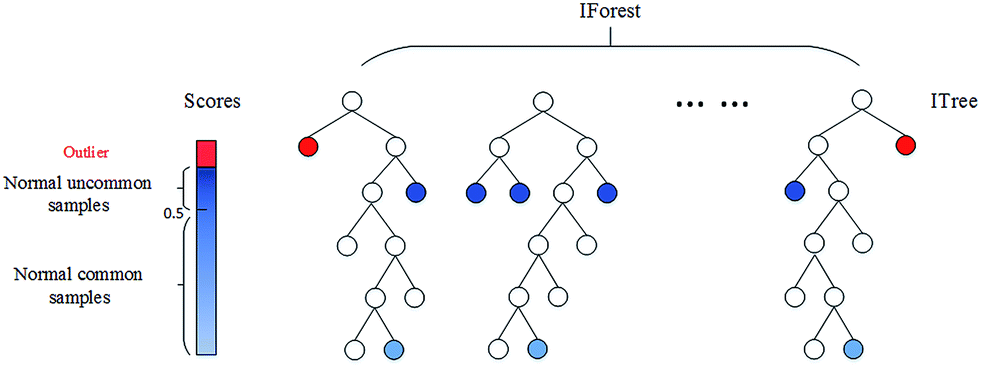
\includegraphics[scale=0.45]{inc/images/iforest-scheme.png}
  \caption{Схема выявления аномалий на основе метода изолирующего леса \cite{Short-outlier-methods-overview}}
  \label{fig:iforest-scheme}
\end{figure}

Основная идея IForest заключается в том, чтобы вычислить оценку аномалии для каждого наблюдения в наборе данных. Для этого строится лес случайных и независимых бинарных изолирующих деревьев (ITree). Также модель использует два входных параметра: размер выборки $\psi$, случайно выбранный из всего набора данных, и $t$ --- количество деревьев в лесу.

\newpage

Построение очередного ITree происходит следующим образом:
\begin{itemize}[leftmargin=0pt,itemindent=4.6em]
    \item инвариант – корневой узел содержит все наблюдения выборки;
    \item IForest случайным образом выбирает подмножество наблюдений $\psi$;
    \item разделение узла $i$: 
        \begin{itemize}[leftmargin=4.6em,itemindent=4.6em]
            \item[$\bullet$] IForest случайным образом выбирает функцию $f_i$  из заданного набора функций;
            \item[$\bullet$] значение разделения $v_i$ также случайным образом выбирается между $\min(f_i)$ и $\max(f_i)$;
            \item[$\bullet$] элементы узла $i$ разбиваются на левую и правую группы (поддеревья) путем сравнения их значений с $v_i$;
        \end{itemize}
    \item процедура разделения рекурсивно продолжается до тех пор, пока все выборочные данные не будут изолированы или дерево не достигнет максимальной глубины, равной $\log_2 \psi$.
\end{itemize}

Так, чтобы построить $t$ изолирующих деревьев леса, необходимо повторить вышеописанные шаги $t$ раз. Построение IForest представляет собой этап обучения в данном методе.

Для каждого наблюдения можно рассчитать показатель выбросов \cite{Isolation-Forest} по формуле (\ref{s_xn_def}):

\begin{equation}\label{s_xn_def}
    s(\overline{x},\ n) = 2^{-\tfrac{\mu(h(x))}{c(n)}},
\end{equation}
где $h(\overline{x})$ --- число шагов до полной изоляции экземпляра $\overline{x}$, \\
$\mu(h(\overline{x}))$ --- среднее значение $h(\overline{x})$, взятое по ансамблю деревьев, \\
$c(n)$ --- значение нормализации, заданное соотношением (\ref{c_n_def}). \\

\begin{equation}\label{c_n_def}
    c(n) = \begin{cases}
         2H(m - 1) - \dfrac{2(m - 1)}{n}, &\ \text{если } m > 2, \\
         1, &\ \text{если } m = 2, \\ 
         0, &\ \text{иначе}, \\ 
    \end{cases}
\end{equation}
где $n$ --- объем данных тестирования, \\
$m$ --- размер набора выборок, \\
$H(i)$ --- число гармоник, которое можно оценить $H(i)=\ln i + \gamma$, где $\gamma \approx 0,577$ --- постоянная Эйлера-Макерони \cite{Eiler-Maskeroni-Const}.

Таким образом, если значение $s(\overline{x}, n)$ близко к $1$, то экземпляр $\overline{x}$ с большой вероятностью является аномалией. Если $s(\overline{x}, n) < \tfrac{1}{2}$, то $\overline{x}$ , скорее всего, относится к нормальной точке выборки.

Данный метод эффективен для обработки больших объемов данных и обладает высокой скоростью обучения, что делает его привлекательным для решения задач обнаружения аномалий в реальном времени. Однако стоит заметить, что в случае локальных выбросов IForest может справляться хуже, чем с глобальными аномалиями.

Более того, в 2023 году в работе \cite{DIF} было представлено новое расширение --- Deep Isolation Forest (DIF). Метод предлагает ряд существенных преимуществ по сравнению со стандартным методом IForest:

\begin{itemize}[leftmargin=0pt,itemindent=4.6em]
    \item[$\bullet$] эффективность в пространствах высокой размерности;
    \item[$\bullet$] избежание алгоритмического смещения (см. рисунок \ref{fig:iforest-and-dif-comparison}): DIF предоставляет более обширный метод изоляции, который может произвольно разделять данные в любом случайном направлении и угле на подпространствах любого размера;
    \item[$\bullet$] возможность обработки сложных и трудноизолируемых аномалий за счёт использования случайных нейронных сетей, не требующих оптимизации.
\end{itemize}

\begin{figure}
  \centering
  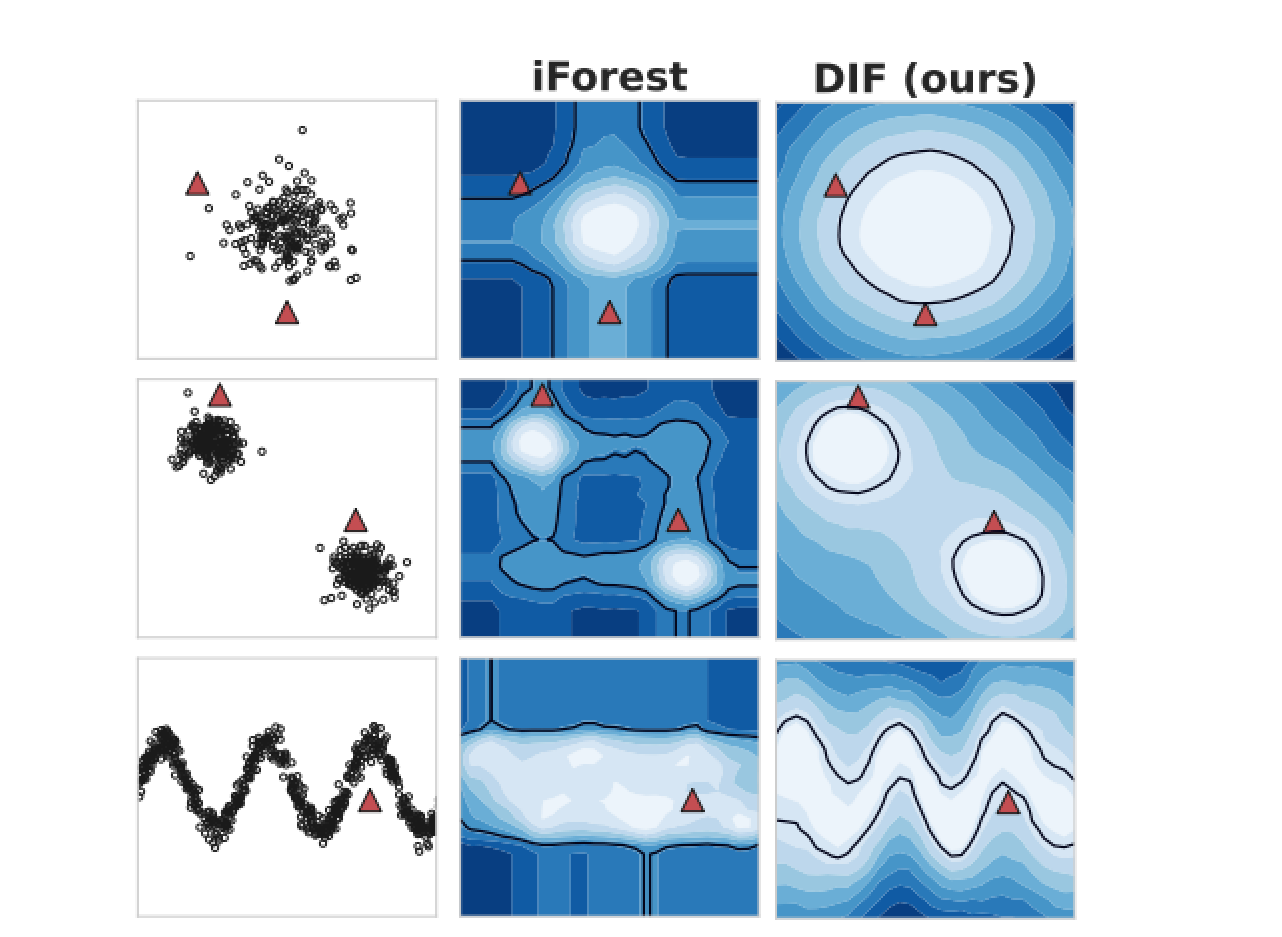
\includegraphics[scale=0.235]{inc/images/iforest-and-dif-comparison.png}
  \caption{Сравнение IForest и DIF: разрешение проблемы алгоритмического смещения при выявлении аномалий \cite{DIF}}
  \label{fig:iforest-and-dif-comparison}
\end{figure}

Таким образом, DIF преодолевает ограничения стандартного IForest, дополняя каноничный метод и предоставляя более гибкое и эффективное средство обнаружения аномалий.

Здесь функция принятия решений $f(\overline{x_i})$ основывается на оценке аномальности $s(\overline{x_i}, n)$, рассчитанной по формуле (\ref{s_xn_def}). Для определения принадлежности экземпляра $\overline{x_i}$ к классу $y_1$ или $y_2$ необходимо установить пороговое значение $s^*$, при превышении которого экземпляр считается аномальным. Таким образом, функция $f(\overline{x_i})$ определяется следующим образом:

\begin{equation}\label{f_iforest_def}
    f(\overline{x_i}) = \begin{cases}
         \ \ 1, &\ \text{если } s(\overline{x_i}, n) \geq s^*, \\
               -1, &\ \text{иначе}.
         \end{cases}
\end{equation}

Выбор порогового значения $s^*$ напрямую влияет на $\alpha$ и $\beta$. Для достижения оптимального баланса между $\alpha$ и $\beta$ необходимо производить калибровку $s^*$ с использованием кросс-валидации.
